\begin{table}[t]
  \caption{Evaluation datasets.}
  \label{tab:datasets}
  \setlength{\tabcolsep}{6pt}
  \renewcommand{\arraystretch}{0.95}
  \begin{tabular}{@{}l l r@{}}
    \hline
    \textbf{Name}                   & \textbf{Type}              & \textbf{Size} \\
    \hline
    \texttt{chr1.pan.smooth.gfa}    & Human chr (smooth)         & 7.1\,GB       \\
    \texttt{chr6.pan.smooth.gfa}    & Human chr (smooth)         & 3.8\,GB       \\
    \texttt{EcoliGraph\_MGC.gfa}    & Microbial (\emph{E. coli}) & 0.113\,GB     \\
    \texttt{hprc-v1.1-mc-chm13.gfa} & Human WGS (HPRC)           & 48\,GB        \\
    \texttt{hprc-v2.0-mc-chm13.gfa} & Human WGS (HPRC)           & 358\,GB       \\
    \texttt{hprc-v2.1-mc-chm13.gfa} & Human WGS (HPRC)           & 369\,GB       \\
    \hline
  \end{tabular}
\end{table}





\aptLtoX[graphic=no,type=html]{\begin{table}[t]
  \caption {Compression ratio, compression (Co.) and decompression (De.) throughput (MB/s) across datasets. {\NoBcBestCr{Blue}} indicates the best performance, {\SecondbestCr{green}} denotes the second best.}
\def\TabDataName#1{\bfseries\scriptsize#1}
%  \newcommand{\TabDataName}[1]{\noindent\rotatebox{90}{\bfseries\scriptsize\scalebox{0.9}{\noindent#1}}}
  \setlength{\tabcolsep}{2pt}
  \renewcommand{\arraystretch}{1.3}
  \resizebox{\columnwidth}{!}{\scriptsize%
\begin{tabular}{l|c|cccccc|cc|}
    \multicolumn{1}{l}{\rotatebox{90}{\textbf{Dataset}}}    &
    \multicolumn{1}{c}{\rotatebox{90}{\textbf{metrics}}}    &
    \multicolumn{1}{c}{\rotatebox{90}{\textbf{Gzip}}}       &
    \multicolumn{1}{c}{\rotatebox{90}{\textbf{Zstd}}}       &
    \multicolumn{1}{c}{\rotatebox{90}{\textbf{sqz}}}        &
    \multicolumn{1}{c}{\rotatebox{90}{\textbf{sqz+bgzip}}}  &
    \multicolumn{1}{c}{\rotatebox{90}{\textbf{sqz+Zstd}}}   &
    \multicolumn{1}{c}{\rotatebox{90}{\textbf{GBZ}}}        &
    \multicolumn{1}{c}{\rotatebox{90}{\textbf{\gfaz(CPU)}}} &
    \multicolumn{1}{c}{\rotatebox{90}{\textbf{\gfaz(GPU)}}}                                                                                                               \\
    \cline{1-2}\cline{3-10}

    \multirow{3}{*}{\TabDataName{chr1.}}                                 & Ratio & 5.59 & 7.54                & 3.09 & 18.0 & 16.7 & 9.52 & \NoBcBestCr{35.4}   & \SecondbestCr{31.7}  \\
                                                                         & Co.   & 46.2 & \SecondbestCr{2178} & 3.95 & 3.97 & 4.00 & 12.1 & 385                 & \NoBcBestCr{2754}    \\
                                                                         & De.   & 359  & 1618                & 21.6 & 21.4 & 21.2 & 284  & \SecondbestCr{1658} & \NoBcBestCr{8124}    \\
    \cline{1-2}\cline{3-10}

    \multirow{3}{*}{\TabDataName{chr6.}}                                 & Ratio & 5.04 & 6.99                & 5.51 & 20.8 & 19.2 & 19.2 & \NoBcBestCr{35.4}   & \SecondbestCr{28.18} \\
                                                                         & Co.   & 41.0 & \SecondbestCr{1712} & 3.56 & 3.56 & 3.59 & 10.7 & 348                 & \NoBcBestCr{3791}    \\
                                                                         & De.   & 348  & 1515                & 20.1 & 20.4 & 20.2 & 281  & \SecondbestCr{1758} & \NoBcBestCr{7230}    \\
    \cline{1-2}\cline{3-10}

    \multirow{3}{*}{\TabDataName{E.coli}}                                & Ratio & 4.69 & 5.67                & 1.26 & 7.46 & 6.79 & 5.58 & \NoBcBestCr{18.3}   & \SecondbestCr{16.7}  \\
                                                                         & Co.   & 33.3 & \NoBcBestCr{1356}   & 4.57 & 4.53 & 4.62 & 20.2 & 190                 & \SecondbestCr{678}   \\
                                                                         & De.   & 310  & \SecondbestCr{1258} & 34.0 & 32.2 & 34.5 & 197  & 491                 & \NoBcBestCr{1430}    \\
    \cline{1-2}\cline{3-10}

    \multirow{3}{*}{\TabDataName{HPRCv1.1}}                              & Ratio & 4.02 & 5.32                & -   & -   & -   & 14.0 & \NoBcBestCr{22.4}   & \SecondbestCr{20.4}  \\
                                                                         & Co.   & 36.4 & \SecondbestCr{1657} & -   & -   & -   & 84.5 & 231                 & \NoBcBestCr{4843}    \\
                                                                         & De.   & 319  & \SecondbestCr{1234} & -   & -   & -   & 650  & 1058                & \NoBcBestCr{9435}    \\
    \cline{1-2}\cline{3-10}

    \multirow{3}{*}{\TabDataName{HPRCv2.0}}                              & Ratio & 4.19 & 6.49                & -   & -   & -   & 66.8 & \NoBcBestCr{83.9}   & \SecondbestCr{76.4}  \\
                                                                         & Co.   & 49.1 & \NoBcBestCr{1514}   & -   & -   & -   & 130  & \SecondbestCr{367}  & -                   \\
                                                                         & De.   & 342  & \SecondbestCr{1240} & -   & -   & -   & 648  & \NoBcBestCr{1652}   & -                   \\
    \cline{1-2}\cline{3-10}

    \multirow{3}{*}{\TabDataName{HPRCv2.1}}                              & Ratio & 4.19 & 6.43                & -   & -   & -   & 64.2 & \NoBcBestCr{82.8}   & \SecondbestCr{74.2}  \\
                                                                         & Co.   & 48.9 & \NoBcBestCr{1540}   & -   & -   & -   & 136  & \SecondbestCr{348}  & -                   \\
                                                                         & De.   & 343  & \SecondbestCr{1241} & -   & -   & -   & 652  & \NoBcBestCr{1559}   & -                   \\
    \cline{1-2}\cline{3-10}
\end{tabular}
  }
  \label{tab:ratio-throughput}
\end{table}}{
\begin{table}[t]
  \caption {Compression ratio, compression (Co.) and decompression (De.) throughput (MB/s) across datasets. {\NoBcBestCr{Blue}} indicates the best performance, {\SecondbestCr{green}} denotes the second best.}
  \newcommand{\TabDataName}[1]{\noindent\rotatebox{90}{\bfseries\scriptsize\scalebox{0.9}{\noindent#1}}}
  \setlength{\tabcolsep}{2pt}
  \scriptsize\color{gray}
  \renewcommand{\arraystretch}{1.3}
  \resizebox{\columnwidth}{!}{%
    \begin{tabular}{>{\color{black}}l|>{\color{black}}c|>{\color{black}}c>{\color{black}}c>{\color{black}}c>{\color{black}}c>{\color{black}}c>{\color{black}}c|>{\color{black}}c>{\color{black}}c|}
    \multicolumn{1}{l}{\rotatebox{90}{\color{black}\textbf{Dataset}}}    &
    \multicolumn{1}{c}{\rotatebox{90}{\color{black}\textbf{metrics}}}    &
    \multicolumn{1}{c}{\rotatebox{90}{\color{black}\textbf{Gzip}}}       &
    \multicolumn{1}{c}{\rotatebox{90}{\color{black}\textbf{Zstd}}}       &
    \multicolumn{1}{c}{\rotatebox{90}{\color{black}\textbf{sqz}}}        &
    \multicolumn{1}{c}{\rotatebox{90}{\color{black}\textbf{sqz+bgzip}}}  &
    \multicolumn{1}{c}{\rotatebox{90}{\color{black}\textbf{sqz+Zstd}}}   &
    \multicolumn{1}{c}{\rotatebox{90}{\color{black}\textbf{GBZ}}}        &
    \multicolumn{1}{c}{\rotatebox{90}{\color{black}\textbf{\gfaz(CPU)}}} &
    \multicolumn{1}{c}{\rotatebox{90}{\color{black}\textbf{\gfaz(GPU)}}}                                                                                                               \\
    \cline{1-2}\cline{3-10}

    \multirow{3}{*}{\TabDataName{chr1.}}                                 & Ratio & 5.59 & 7.54                & 3.09 & 18.0 & 16.7 & 9.52 & \NoBcBestCr{35.4}   & \SecondbestCr{31.7}  \\
                                                                         & Co.   & 46.2 & \SecondbestCr{2178} & 3.95 & 3.97 & 4.00 & 12.1 & 385                 & \NoBcBestCr{2754}    \\
                                                                         & De.   & 359  & 1618                & 21.6 & 21.4 & 21.2 & 284  & \SecondbestCr{1658} & \NoBcBestCr{8124}    \\
    \cline{1-2}\cline{3-10}

    \multirow{3}{*}{\TabDataName{chr6.}}                                 & Ratio & 5.04 & 6.99                & 5.51 & 20.8 & 19.2 & 19.2 & \NoBcBestCr{35.4}   & \SecondbestCr{28.18} \\
                                                                         & Co.   & 41.0 & \SecondbestCr{1712} & 3.56 & 3.56 & 3.59 & 10.7 & 348                 & \NoBcBestCr{3791}    \\
                                                                         & De.   & 348  & 1515                & 20.1 & 20.4 & 20.2 & 281  & \SecondbestCr{1758} & \NoBcBestCr{7230}    \\
    \cline{1-2}\cline{3-10}

    \multirow{3}{*}{\TabDataName{E.coli}}                                & Ratio & 4.69 & 5.67                & 1.26 & 7.46 & 6.79 & 5.58 & \NoBcBestCr{18.3}   & \SecondbestCr{16.7}  \\
                                                                         & Co.   & 33.3 & \NoBcBestCr{1356}   & 4.57 & 4.53 & 4.62 & 20.2 & 190                 & \SecondbestCr{678}   \\
                                                                         & De.   & 310  & \SecondbestCr{1258} & 34.0 & 32.2 & 34.5 & 197  & 491                 & \NoBcBestCr{1430}    \\
    \cline{1-2}\cline{3-10}

    \multirow{3}{*}{\TabDataName{HPRCv1.1}}                              & Ratio & 4.02 & 5.32                & -   & -   & -   & 14.0 & \NoBcBestCr{22.4}   & \SecondbestCr{20.4}  \\
                                                                         & Co.   & 36.4 & \SecondbestCr{1657} & -   & -   & -   & 84.5 & 231                 & \NoBcBestCr{4843}    \\
                                                                         & De.   & 319  & \SecondbestCr{1234} & -   & -   & -   & 650  & 1058                & \NoBcBestCr{9435}    \\
    \cline{1-2}\cline{3-10}

    \multirow{3}{*}{\TabDataName{HPRCv2.0}}                              & Ratio & 4.19 & 6.49                & -   & -   & -   & 66.8 & \NoBcBestCr{83.9}   & \SecondbestCr{76.4}  \\
                                                                         & Co.   & 49.1 & \NoBcBestCr{1514}   & -   & -   & -   & 130  & \SecondbestCr{367}  & -                   \\
                                                                         & De.   & 342  & \SecondbestCr{1240} & -   & -   & -   & 648  & \NoBcBestCr{1652}   & -                   \\
    \cline{1-2}\cline{3-10}

    \multirow{3}{*}{\TabDataName{HPRCv2.1}}                              & Ratio & 4.19 & 6.43                & -   & -   & -   & 64.2 & \NoBcBestCr{82.8}   & \SecondbestCr{74.2}  \\
                                                                         & Co.   & 48.9 & \NoBcBestCr{1540}   & -   & -   & -   & 136  & \SecondbestCr{348}  & -                   \\
                                                                         & De.   & 343  & \SecondbestCr{1241} & -   & -   & -   & 652  & \NoBcBestCr{1559}   & -                   \\
    \cline{1-2}\cline{3-10}
\end{tabular}
  }
  \label{tab:ratio-throughput}
\end{table}}


\section{Evaluation}\label{sec:evaluation}

\subsection{Experimental Setup}\label{subsec:setup}

All experiments run on a workstation with an AMD Ryzen Threadripper PRO 9955WX (16 cores), an NVIDIA RTX Pro 6000 GPU, and 512\,GB of DDR5 6400 MHz memory.
For CPU compressors that support multithreading, we enable all 16 hardware threads.
Unless otherwise noted, \texttt{zstd} uses compression level 9.
To measure algorithmic throughput rather than storage performance, we report \emph{warm-cache} timings averaged over 5 runs: before each run, we prime the OS page cache by streaming the input file once (e.g., \texttt{cat input.gfa > /dev/null}) to minimize disk I/O effects.

\subsection{Dataset}\label{subsec:dataset}
We evaluate our compressor on the datasets summarized in Table~\ref{tab:datasets}.
For readability, we refer to the chromosome-scale smoothed graphs using short names
(\texttt{chr1.pan.\allowbreak smooth.gfa} and \texttt{chr6.pan.\allowbreak smooth.gfa})~\cite{hpp_data_portal}.
These datasets are representative for three reasons. The chromosome scale PGGB graphs (chr1/chr6) provide realistic human pangenome structure at a manageable scale, making it easier to stress specific components (e.g., traversal redundancy) without the full whole-genome footprint.
Second, the HPRC minigraph--cactus graphs span multiple rapidly evolving public releases (v1.1, v2.0, v2.1)~\cite{hpp_data_portal}, allowing us to evaluate robustness as graph construction pipelines and graph complexity change over time.
Finally, \texttt{EcoliGraph\_MGC.gfa}~\cite{DO1RTF_2025} tests generality beyond human genomes on a microbial pangenome with dense path sets and different repeat/variation characteristics.






\begin{figure*}[t]
  \centering
  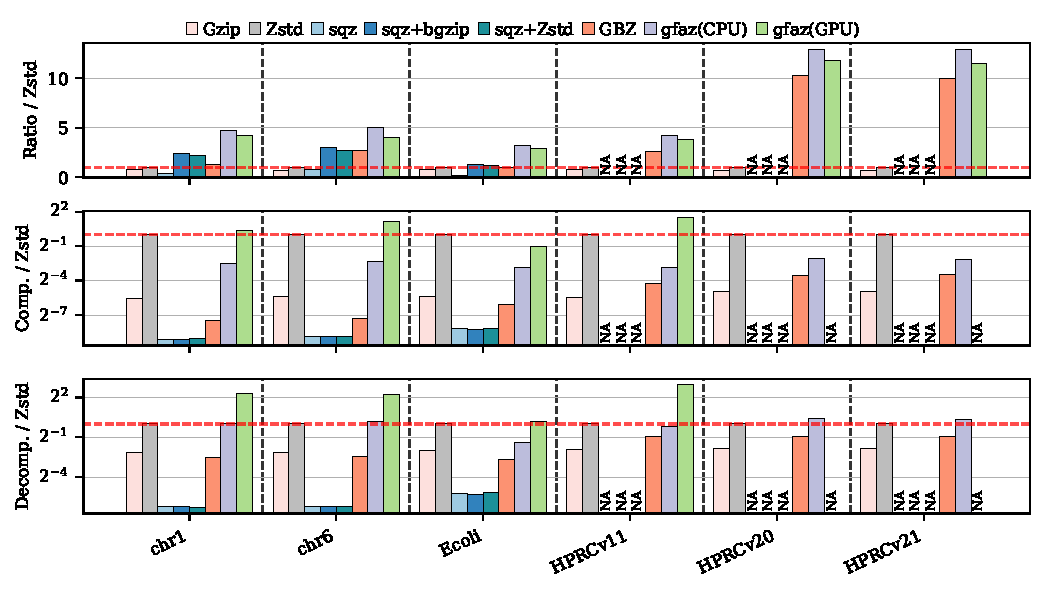
\includegraphics[width=\linewidth]{fig_eval_norm_combined.pdf}
  \caption{Normalized compression ratio, compression speed, and decompression speed relative to Zstd across all datasets. Results are normalized such that Zstd = 1.0 (dashed horizontal line). Speed metrics are plotted on a log scale (base 2).}
  \label{fig:eval-norm}
\end{figure*}


\begin{figure*}[t]
  \centering
  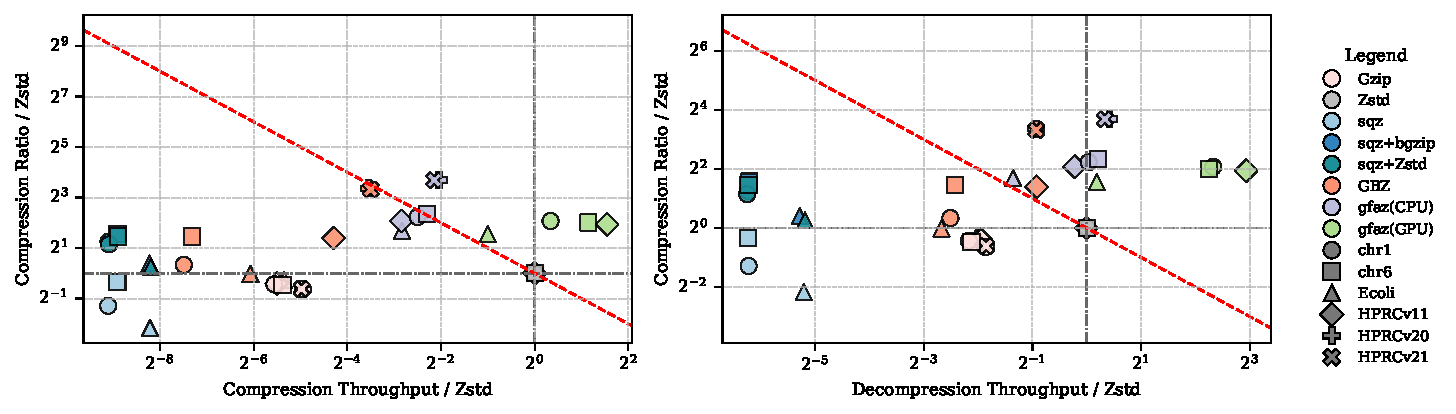
\includegraphics[width=\linewidth]{fig_pareto_combined.pdf}
  \caption{Pareto trade-off between compression ratio (y-axis) and speed (x-axis), normalized to Zstd (baseline at $1.0$). The dashed diagonal line ($y=1/x$) represents an iso-efficiency curve where a $2\times$ increase in ratio compensates for a $2\times$ drop in speed. Points above this line and to the right represent better trade-offs than the baseline.}
  \label{fig:pareto}
\end{figure*}


\begin{table*}[t]
  \centering
  \scriptsize
  \setlength{\tabcolsep}{3pt}
  \renewcommand{\arraystretch}{1.05}
  \caption{Ablation of \texttt{Compact} and \texttt{Sort} on rulebook effectiveness.
    Each cell shows \(H\) / \(L\), where \(H=r\gg32\) and \(L=r\,\&\,\texttt{0xffffffff}\); each entry is the ZSTD-compressed size followed by the compression ratio in parentheses.}
  \label{tab:compact-sort-ablation}
  \resizebox{\textwidth}{!}{%
    \setlength{\tabcolsep}{2pt}
\begin{tabular}{l|c|c|c|c}
  \hline
  \textbf{Dataset}    & \textbf{compact+sort} & \textbf{compact} & \textbf{sort} & \textbf{none} \\
  \hline
  EcoliGraph\_MGC     &
  53.9\,KB (\textbf{9.6$\times$}) / 215\,KB (\textbf{2.4$\times$})    &
  348\,KB (1.5$\times$) / 358\,KB (1.4$\times$)                       &
  70.7\,KB (9.6$\times$) / 291\,KB (2.3$\times$)                      &
  463\,KB (1.5$\times$) / 477\,KB (1.4$\times$)                       \\
  chr1.pan.smooth     &
  4.3\,MB (\textbf{11.2$\times$}) / 30.4\,MB (\textbf{1.6$\times$})   &
  40.6\,MB (1.2$\times$) / 40.6\,MB (1.2$\times$)                     &
  5.2\,MB (11.1$\times$) / 38.0\,MB (1.5$\times$)                     &
  50.0\,MB (1.2$\times$) / 50.0\,MB (1.2$\times$)                     \\
  chr6.pan.smooth     &
  2.0\,MB (\textbf{12.1$\times$}) / 14.0\,MB (\textbf{1.7$\times$})   &
  19.3\,MB (1.2$\times$) / 19.3\,MB (1.2$\times$)                     &
  2.4\,MB (12.0$\times$) / 17.8\,MB (1.6$\times$)                     &
  24.1\,MB (1.2$\times$) / 24.1\,MB (1.2$\times$)                     \\
  hprc-v1.1           &
  61.2\,MB (\textbf{10.2$\times$}) / 330\,MB (\textbf{1.9$\times$})   &
  565\,MB (1.1$\times$) / 561\,MB (1.1$\times$)                       &
  73.9\,MB (10.4$\times$) / 418\,MB (1.8$\times$)                     &
  697\,MB (1.1$\times$) / 692\,MB (1.1$\times$)                       \\
  hprc-v2.0           &
  124\,MB (\textbf{13.1$\times$}) / 1254\,MB (\textbf{1.3$\times$})   &
  1512\,MB (1.1$\times$) / 1513\,MB (1.1$\times$)                     &
  153\,MB (13.0$\times$) / 1558\,MB (1.3$\times$)                     &
  1857\,MB (1.1$\times$) / 1859\,MB (1.1$\times$)                     \\
  hprc-v2.1           &
  130\,MB (\textbf{13.1$\times$}) / 1315\,MB (\textbf{1.3$\times$})   &
  1588\,MB (1.1$\times$) / 1589\,MB (1.1$\times$)                     &
  161\,MB (12.9$\times$) / 1632\,MB (1.3$\times$)                     &
  1949\,MB (1.1$\times$) / 1951\,MB (1.1$\times$)                     \\
  \hline
\end{tabular}

  }
\end{table*}



\subsection{Compression-Decompression Performance}\label{subsec:compression-performance}

We include gzip and zstd as general-purpose baselines, GBZ and SQZ as pangenome-oriented compressors; for SQZ we also report \texttt{sqz+bgzip} and \texttt{sqz+zstd} to probe its best ratio under alternative back-end compressors.
SQZ runs out of memory on HPRC v1.1 and larger graphs, so those entries are marked NA.
SQZ and GBZ also drop parts of the original GFA representation, making the \gfaz comparisons conservative.
For the 300+\,GB HPRC v2.0/v2.1 graphs, the current GPU implementation runs out of device memory; we therefore report GPU ratios via a CPU simulation of the GPU rule-mining/encoding logic and omit GPU throughput for those two datasets.
Table~\ref{tab:ratio-throughput} reveals three consistent patterns.


\noindent \textbf{Insight 1 (ratio gains increase with graph complexity).}
\gfaz gives the best ratio on all datasets with available results, for both backends. On chr1, \gfaz(CPU) reaches 35.4$\times$ versus zstd 7.54$\times$ and GBZ 9.52$\times$; on chr6, 35.4$\times$ versus 6.99$\times$ and 19.2$\times$.
On larger HPRC graphs, the gap widens: on v2.0, \gfaz(CPU) reaches 83.9$\times$ versus zstd 6.49$\times$ and GBZ 66.8$\times$; on v2.1, 82.8$\times$ versus 6.43$\times$ and 64.2$\times$.
The GPU ratio is consistently but modestly below CPU (e.g., 31.7$\times$ vs 35.4$\times$ on chr1, 20.4$\times$ vs 22.4$\times$ on v1.1), consistent with checkerboard encoding (Section~\ref{subsec:gpu}) replacing fewer overlapping opportunities than serial greedy encoding in each round.
The ratio advantage is not specific to the HPRC pipeline. Table~\ref{tab:ratio-other} adds two graphs from other sources: HGSVC3, an $80.1$\,GB whole-genome Minigraph--Cactus pangenome from a different consortium, and a chromosome from the 1000-genome-scale 1KCP collection whose variation is carried entirely in graph topology (a reference-only GFA with no embedded haplotype paths). On both, \gfaz(CPU) again gives by far the best ratio---$28.1\times$ on HGSVC3 and $18.4\times$ on 1KCP-chr1, versus $4.0$--$4.5\times$ for gzip and $6.9$--$7.1\times$ for zstd.

\begin{table}[t]
\centering
\caption{Compression ratio on two graphs from outside the HPRC (single-run, ratio only). \gfaz retains its ratio advantage on a different-consortium pangenome (HGSVC3) and on a topology-only graph (1KCP-chr1).}
\label{tab:ratio-other}
\small
\begin{tabular}{lrrrr}
\hline
Dataset & GFA & Gzip & Zstd & \gfaz(CPU) \\
\hline
HGSVC3      & 80.1\,GB & 4.0$\times$ & 7.1$\times$ & \textbf{28.1$\times$} \\
1KCP-chr1   & 1.66\,GB & 4.5$\times$ & 6.9$\times$ & \textbf{18.4$\times$} \\
\hline
\end{tabular}
\end{table}

\noindent \textbf{Insight 2 (Throughput remains strong across CPU/GPU).}
When inputs fit GPU memory, \gfaz(GPU) is the fastest high-ratio operating point: on HPRC v1.1, it reaches 4843/9435 MB/s compression/decompression, versus \gfaz(CPU) at 231/1058 MB/s and zstd at 1657/1234 MB/s.
On chr1 and chr6, \gfaz(GPU) also leads throughput, showing that the GPU backend is most effective when traversal data can remain device-resident.
For v2.0/v2.1, GPU throughput is unavailable because the traversal stream exceeds device memory, but \gfaz(CPU) still gives the fastest decompression (1652 and 1559 MB/s) while retaining much higher ratios than zstd.
CPU compression is slower than zstd on these largest graphs, but this trade-off is favorable for storage and repeated-read workloads.
On the small \emph{E. coli} input, zstd compresses fastest, while \gfaz(GPU) still improves both ratio and decompression speed.

\noindent \textbf{Insight 3 (alternative methods occupy weaker ratio--speed fronts).}
SQZ variants can improve ratio over gzip/zstd on chromosome graphs, but their throughput (about 3--5 MB/s compression and about 20--35 MB/s decompression) is two orders of magnitude lower than \gfaz.
GBZ is the strongest non-\gfaz ratio baseline on large HPRC graphs, but remains below \gfaz in ratio (66.8$\times$/64.2$\times$ vs 83.9$\times$/82.8$\times$ on v2.0/v2.1) and decompression speed (648/652 vs 1652/1559 MB/s on CPU), while preserving fewer GFA semantics.

\begin{table}[t]
  \centering
  \scriptsize
  \setlength{\tabcolsep}{3pt}
  \renewcommand{\arraystretch}{1.05}
  \caption{Random-access evaluation using \texttt{extract-traversal}. We measure the time and peak memory required to reconstruct only 1, 4, or 16 selected paths/walks from an existing \texttt{.gfaz} file.}
  \label{tab:random-access}
  \resizebox{\columnwidth}{!}{%
    \begin{tabular}{lrrrr}
      \hline
      \textbf{Dataset} & \textbf{Extracted} & \textbf{Elapsed (s)} & \textbf{Peak Mem. (GB)} & \textbf{GFA Size (GB)} \\
      \hline
      \multirow{3}{*}{chr1}       & 1  & 0.102 & 0.38 & 7.1 \\
                                   & 4  & 0.103 & 0.37 & 7.1 \\
                                   & 16 & 0.106 & 0.41 & 7.1 \\
      \hline
      \multirow{3}{*}{hprc-v1.1}  & 1  & 1.006 & 4.09 & 48 \\
                                   & 4  & 1.012 & 4.10 & 48 \\
                                   & 16 & 1.029 & 4.13 & 48 \\
      \hline
      \multirow{3}{*}{hprc-v2.0}  & 1  & 2.285 & 9.26 & 358 \\
                                   & 4  & 2.302 & 9.28 & 358 \\
                                   & 16 & 2.312 & 9.30 & 358 \\
      \hline
      \multirow{3}{*}{hprc-v2.1}  & 1  & 2.278 & 9.65 & 369 \\
                                   & 4  & 2.303 & 9.67 & 369 \\
                                   & 16 & 2.380 & 9.74 & 369 \\
      \hline
    \end{tabular}
  }
\end{table}

\begin{table}[t]
  \centering
  \scriptsize
  \setlength{\tabcolsep}{5pt}
  \renewcommand{\arraystretch}{1.05}
  \caption{Incremental haplotype extension using \texttt{add-haplotypes}. Each run appends 50 new paths/walks using the rulebook already stored in the input \texttt{.gfaz} file.}
  \label{tab:incremental-extension}
  \resizebox{\columnwidth}{!}{%
    \begin{tabular}{lrrrr}
      \hline
      \textbf{Dataset} & \textbf{Added Haplotypes} & \textbf{Elapsed (s)} & \textbf{Peak Memory (GB)} & \textbf{GFA Size (GB)} \\
      \hline
      chr1       & 50 & 0.95  & 0.97  & 7.1 \\
      chr6       & 50 & 0.54  & 0.51  & 3.8 \\
      hprc-v1.1  & 50 & 3.25  & 3.25  & 48 \\
      hprc-v2.0  & 50 & 9.80  & 16.85 & 358 \\
      hprc-v2.1  & 50 & 10.20 & 17.32 & 369 \\
      \hline
    \end{tabular}
  }
\end{table}




\noindent \textbf{Normalized and Pareto views.}
Figures~\ref{fig:eval-norm} and~\ref{fig:pareto} summarize the same results normalized to Zstd. \gfaz consistently improves decompression and ratio efficiency.
For compression, only the small input can fall below the line but still keeps a substantial multi-fold ratio advantage over Zstd.



\subsection{Random Access and Incremental Extension}\label{subsec:random-access-eval}

We next evaluate the two traversal-centric operations enabled by the \texttt{.gfaz} layout: extracting a small number of haplotypes without full decompression, and appending new haplotypes without recompressing the entire file.

\noindent \textbf{Random access.}
Table~\ref{tab:random-access} reports extraction of 1, 4, or 16 paths/walks from existing \texttt{.gfaz} files. Runtime stays nearly flat as more records are requested. On HPRC v2.1 (369\,GB), extracting 1, 4, and 16 haplotypes takes 2.28\,s, 2.30\,s, and 2.38\,s, respectively. Peak memory also changes only slightly, from 9.65\,GB to 9.74\,GB.

\noindent \textbf{Incremental extension.}
Table~\ref{tab:incremental-extension} reports the cost of appending 50 new haplotypes. This takes 0.54--0.95\,s on chromosome-scale graphs, 3.25\,s on HPRC v1.1, and about 10\,s on the 358--369\,GB graphs. On HPRC v2.1, appending 50 haplotypes takes 10.2\,s, compared with roughly 1100\,s for full recompression.



\subsection{Ablation: Compact and Sort}\label{subsec:ablation-compact-sort}
We evaluate four workflow variants: \texttt{compact+sort} (full design), \texttt{compact} only, \texttt{sort} only, and \texttt{none}.
For each packed 64-bit rule ID \(r\), we split it into two 32-bit integer streams:
\(H = r \gg 32\) (high 32 bits) and \(L = r \,\&\, \texttt{0xffffffff}\) (low 32 bits) during compression, then entropy-code each stream with ZSTD.
Results directly validate the design rationale in Section~\ref{subsec:pipeline}.
Sorting is the dominant factor for \(H\): on chr1, \(H\) improves from 1.2$\times$ (\texttt{none}) to 11.1$\times$ (\texttt{sort}), and to 11.2$\times$ with \texttt{compact+sort}; similarly on hprc-v2.1, 1.1$\times$ (\texttt{none}) to 12.9$\times$ (\texttt{sort}) and 13.1$\times$ (\texttt{compact+sort}).
Compact then provides additional gains by removing unused rules and shrinking emitted streams: for chr1 \(L\) improves from 1.5$\times$ (\texttt{sort}) to 1.6$\times$ (\texttt{compact+sort}), and for hprc-v2.1 from 1.3$\times$ to 1.3$\times$ with a concrete size drop (1632\,MB to 1315\,MB).
Compared with \texttt{compact} only, the full \texttt{compact+sort} pipeline is consistently much better on \(H\) (e.g., chr6: 12.1$\times$ vs 1.2$\times$), showing that compacting without ordering does not create enough entropy structure for the rulebook.
This also clarifies a weakness of SQZ: although SQZ is grammar-based, highly variable rule symbols without strong ordering reduce rule-stream regularity, making entropy coding less effective than the sorted rulebook layout used by \gfaz.


\begin{table}[t]
  \centering
  \scriptsize
  \setlength{\tabcolsep}{4pt}
  \renewcommand{\arraystretch}{1.05}
  \caption{CPU stage-level profiling for compression and decompression.
    Share is computed as \texttt{time / stage total}.}
  \label{tab:cpu-breakdown}
  \resizebox{\columnwidth}{!}{%
    \setlength{\tabcolsep}{2pt}
\begin{tabular}{l r r r}
  \hline
  \textbf{Stage}                     & \textbf{Time (ms)} & \textbf{Tput (GB/s)} & \textbf{Share} \\
  \hline
  \multicolumn{4}{l}{\textit{Compression (total: 19888.78\,ms)}}                                  \\
  Grammar subtotal                   & 11004.68            & 0.20                  & 55.3\%         \\
  \quad generate\_rules              & 6000.89             & 0.38                  & 30.2\%         \\
  \quad encode\_traversals           & 4785.13             & 0.47                  & 24.1\%         \\
  \quad compact\_sort\_remap         & 196.83              & 11.5                  & 1.0\%          \\
  \quad split+delta\_encode          & 27.93               & 3.30                  & 0.1\%          \\
  \quad zstd compress                & 467.58              & 0.47                  & 2.4\%          \\
  Others                             & 8884.10             & --                    & 44.7\%         \\
  \hline
  \multicolumn{4}{l}{\textit{Decompression (total: 4221.47\,ms)}}                                 \\
  Grammar subtotal                   & 511.52              & 4.32                  & 12.1\%         \\
  \quad zstd decompress              & 102.39              & 1.60                  & 2.4\%          \\
  \quad decode rules (prefix sum)    & 2.85                & 32.4                  & 0.1\%          \\
  \quad expand traversals            & 371.93              & 6.06                  & 8.8\%          \\
  \quad decode traversals (pfx sum)  & 34.35               & 65.6                  & 0.8\%          \\
  Others                             & 3709.95             & --                    & 87.9\%         \\
  \hline
\end{tabular}

  }
\end{table}

\begin{table}[t]
  \centering
  \scriptsize
  \setlength{\tabcolsep}{4pt}
  \renewcommand{\arraystretch}{1.05}
  \caption{GPU stage-level profiling for compression and decompression.
    Share is computed as \texttt{time / stage total}.}
  \label{tab:gpu-breakdown}
  \resizebox{\columnwidth}{!}{%
    \setlength{\tabcolsep}{2pt}
\begin{tabular}{l r r r}
  \hline
  \textbf{Stage}                     & \textbf{Time (ms)} & \textbf{Tput (GB/s)} & \textbf{Share} \\
  \hline
  \multicolumn{4}{l}{\textit{Compression (total: 2322.85\,ms)}}                                   \\
  Grammar subtotal                   & 571.85              & 3.96                  & 24.6\%         \\
  \quad find\_max\_abs               & 5.96                & 378.0                 & 0.3\%          \\
  \quad delta\_encode                & 5.64                & 400.0                 & 0.2\%          \\
  \quad find\_repeated\_2mers        & 195.59              & 11.5                  & 8.4\%          \\
  \quad create\_rule\_table          & 18.36               & 122.8                 & 0.8\%          \\
  \quad apply\_2mer\_rules           & 105.24              & 21.4                  & 4.5\%          \\
  \quad compact\_rules\_remap        & 25.68               & 87.8                  & 1.1\%          \\
  \quad sort\_rules\_remap           & 16.70               & 135.0                 & 0.7\%          \\
  \quad split+delta\_encode          & 0.90                & 102.2                 & 0.0\%          \\
  \quad Zstd compress (nvComp)       & 197.78              & 11.4                  & 8.5\%          \\
  Others                             & 1751.00             & --                    & 75.4\%         \\
  \hline
  \multicolumn{4}{l}{\textit{Decompression (total: 876.00\,ms)}}                                  \\
  Grammar subtotal                   & 117.00              & 19.3                  & 13.4\%         \\
  \quad Zstd decompress (nvComp)     & 85.85               & 26.3                  & 9.8\%          \\
  \quad decode rules (prefix sum)    & 0.44                & 367.2                 & 0.1\%          \\
  \quad expand traversals            & 24.73               & 91.2                  & 2.8\%          \\
  \quad decode traversals (pfx sum)  & 5.98                & 377.1                 & 0.7\%          \\
  Others                             & 759.00              & --                    & 86.6\%         \\
  \hline
\end{tabular}

  }
\end{table}



\begin{table}[t]
  \centering
  \scriptsize
  \setlength{\tabcolsep}{3pt}
  \renewcommand{\arraystretch}{1.05}
  \caption{CPU peak resident memory using 16 threads for compression, a legacy decompression baseline that fully materializes the in-memory \texttt{GfaGraph}, and the implemented streaming decompression path.}
  \label{tab:cpu-memory}
  \resizebox{\columnwidth}{!}{%
    \begin{tabular}{lrrrr}
      \hline
      \textbf{Dataset} & \textbf{Comp.} & \textbf{Full-Graph} & \textbf{Streaming} & \textbf{GFA} \\
      \textbf{} & \textbf{Peak (GB)} & \textbf{Decomp. (GB)} & \textbf{Decomp. (GB)} & \textbf{Size (GB)} \\
      \hline
      chr1       & 7.4   & 6.3   & 0.98 & 7.1 \\
      chr6       & 3.2   & 3.0   & 0.66 & 3.8 \\
      Ecoli      & 0.24  & 0.18  & 0.18 & 0.113 \\
      hprc-v1.1  & 45    & 37    & 3.4  & 48 \\
      hprc-v2.0  & 343   & 289   & 19.3 & 358 \\
      hprc-v2.1  & 356   & 295   & 20.7 & 369 \\
      \hline
    \end{tabular}
  }
\end{table}



\subsection{Performance Breakdown}\label{subsec:breakdown}
Tables~\ref{tab:gpu-breakdown} and~\ref{tab:cpu-breakdown} break down stage-level profiling for the GPU and CPU backends respectively. Each table reports a \texttt{Grammar subtotal} (traversal-related stages) and \texttt{Others} (all remaining fields---segment sequences, link/jump/containment columns, optional fields, and their associated ZSTD encoding).

On both backends, decompression is dominated by \texttt{Others}: 87.9\% on CPU and 86.6\% on GPU, leaving only 12.1\% (CPU) and 13.4\% (GPU) in grammar stages.
Within grammar decode, traversal expansion itself is fast (371.93\,ms at 6.06\,GB/s on CPU; 24.73\,ms at 91.2\,GB/s on GPU), consistent with one-pass expansion and \(O(1)\) rule lookup (\texttt{rule\_id - min\_rule\_id}).
This supports the design claim that traversal reconstruction is not the end-to-end bottleneck once the rulebook is available.

The two backends differ mainly in compression cost distribution.
On CPU, grammar stages consume 55.3\% of compression time, with \texttt{generate\_rules} (30.2\%) and \texttt{encode\_traversals} (24.1\%) as dominant kernels.
On GPU, grammar drops to 24.6\% of total compression time (\texttt{find\_repeated\_2mers} 8.4\%, \texttt{apply\_2mer\_rules} 4.5\%), while \texttt{Others} rises to 75.4\%, consistent with nvComp/ZSTD orchestration overhead in the current pipeline.
This profile explains why the GPU grammar algorithm is already fast but end-to-end speedups are now limited by entropy and non-traversal stages.

\subsection{CPU Memory Profiling}\label{subsec:cpu-memory}

Table~\ref{tab:cpu-memory} compares three CPU memory profiles measured with 16 threads: compression, a legacy decompression baseline that fully materializes the entire \texttt{GfaGraph}, and the implemented streaming decompression path that expands one path/walk and writes it out immediately. The fully materialized baseline reaches 37\,GB, 289\,GB, and 295\,GB on HPRC v1.1, v2.0, and v2.1, respectively. In contrast, the implemented streaming path reduces peak decompression memory to 3.4\,GB, 19.3\,GB, and 20.7\,GB, a reduction of about \(14\text{--}15\times\).

High compression peak memory is less critical in practice for three reasons. First, it occurs primarily in the first rule-encoding round and drops quickly afterward as the traversal stream shrinks. Second, compression is usually a one-time preprocessing step, whereas decompression and downstream analyses are run repeatedly. Third, downstream graph tools such as VG~\cite{garrison2018variation} and ODGI~\cite{guarracino2022odgi} already require memory footprints larger than the input GFA size.
